
% SECTION 5: EXPLAINABILITY (XAI)

\section{Explainability and Clinical Trustworthiness}
\label{sec:xai}

State-of-the-art performance on benchmark datasets does not by itself, justify clinical deployment. As deep learning architectures approach diagnostic parity with specialist radiologists in renal imaging tasks, the central question has shifted from \textit{how accurate?} to \textit{how trustworthy?} Explainable AI (XAI) sits at the heart of this transition: it provides the interpretive scaffolding through which complex model decisions can be audited, validated, and ultimately trusted by the clinicians who act on them. This section examines why transparency is a non-negotiable requirement in nephrology-oriented AI, evaluates the practical landscape of post-hoc visualization and inherently interpretable design, and considers how these tools together support a collaborative, human-in-the-loop clinical workflow.

\subsection{Why Explainability Matters in Surgical Planning}
\label{subsec:why_xai}

High Dice scores and classification accuracies are necessary but insufficient criteria for surgical AI. In nephrology, automated output directly shape high-stakes procedural decisions from preoperative planning for Percutaneous Nephrolithotomy (PCNL) to intraoperative guidance during robot-assisted partial nephrectomies~\cite{li2022automatic}. Under these conditions, an unexplained prediction carries genuine clinical risk: if a model flags a renal mass without indicating which imaging features drove that classification, the clinician has no reliable means to confirm or contest it~\cite{kadhim2024machine}.

This accountability gap is not merely philosophical. A comparative study on stone-free rate prediction demonstrated that large language models, despite their broad linguistic capabilities, failed to outperform validated clinical scoring systems precisely because their reasoning chains were opaque and could not be subjected to clinical scrutiny~\cite{elmaagac2026comparison}. The authors identified non-transparency as a primary barrier to adoption--a finding that generalises across deep learning modalities in urological AI. XAI addresses this by transforming black-box predictions into auditable, spatially grounded justifications, repositioning automated systems as decision-support tools rather than autonomous diagnostic agents.

\subsection{Gradient-Based Visualizations: Grad-CAM and Variants}
\label{subsec:gradcam}

Gradient-weighted Class Activation Mapping (Grad-CAM) remains the most widely adopted post-hoc interpretability technique in renal imaging, owing to its architectural agnosticism and low implementation overhead. By back-projecting the spatial gradients of the final convolutional layer onto the input image, Grad-CAM generates coarse localization heatmaps that identify the anatomical regions most influential to a given prediction. In CT-based renal analysis, this mechanism offers clinicians a rapid visual sanity check: does the model's activation align with the pathological region, or is it responding to irrelevant background structure?

Multi-center 3D CNN frameworks have leveraged these maps to establish explainable visual correlations between lesion size and detection confidence across heterogeneous imaging protocols~\cite{liang2025multicenter}. Attention-augmented detectors similarly employ spatial and channel attention outputs to confirm that network focus concentrates on calcified stone deposits or irregular tumor margins rather than adjacent parenchymal tissue~\cite{sajid2026yolov8}. The DAE-Former architecture goes a step further, demonstrating that Transformer-based attention maps can be inherently gradient-interpretable, providing multi-organ contouring outputs with built-in spatial accountability for radiation dose planning~\cite{azad2023daeformer}.

Nonetheless, gradient-based explanations carry well-documented limitations. Their spatial resolution is constrained by the receptive field of the final convolutional stage, and they are susceptible to highlighting imaging features that are statistically correlated with the target class without being causally responsible for the pathology. This distinction---correlation versus causation in saliency mapping---remains an open research problem and motivates the exploration of more structurally integrated interpretability approaches.


\subsection{Inherent Interpretability vs.\ Post-Hoc Analysis}
\label{subsec:inherent_vs_posthoc}

Post-hoc methods like Grad-CAM and SHAP (SHapley Additive exPlanations) offer broad applicability across pre-trained networks, but their explanations are approximations of decisions already made. A fundamentally different design philosophy embeds interpretability into the architecture itself, ensuring that the reasoning process is transparent by construction rather than reconstructed after the fact.

Convolutional Block Attention Modules (CBAM) and Bi-Level Routing Attention (BRA), as deployed in hybrid CNN-Transformer segmentation networks, produce explicit spatial focus matrices at each feature extraction stage~\cite{lan2024braunet}. The practical implication is that a radiologist reviewing such a model's output can trace exactly which spatial regions were weighted at each processing layer, rather than relying on a single terminal heatmap. This architectural transparency is particularly valuable in multi-class scenarios: in the CNN-Attention-LSTM framework for sequential kidney stone detection, the integrated attention outputs identify high-activation stone positions slice-by-slice, constructing an auditable diagnostic chain across volumetric CT series~\cite{alebada2026hybrid}.

At the other end of the interpretability spectrum, classical feature engineering approaches---such as Gray-Level Co-occurrence Matrix (GLCM) texture analysis combined with statistical feature selection (POE+ACC)---offer fully deterministic, rule-based transparency~\cite{farjad2021ct}. This drive for architectural transparency, alternative structured feature extraction, and domain-adapted text-vision models is similarly documented across a wide swath of earlier computational frameworks and hybrid benchmarks~\cite{hossain2024adaptive, elton2022deep, lee2020biobert, fang2023bioformer, luo2022biogpt, hatsutani2023protuberance, sharma2025hybrid, martin2025evaluation}. These methods produce inherently interpretable decision boundaries but sacrifice the semantic depth and contextual sensitivity that deep representations provide. In practice, neither extreme is universally optimal; the appropriate balance depends on the clinical task, the regulatory environment, and the degree of radiologist oversight available. Hybrid approaches that pair deep visual features with structured, interpretable output heads represent the most pragmatic direction for near-term clinical deployment.

\subsection{Human-AI Collaboration and Standardisation}
\label{subsec:human_ai}

The practical goal of XAI in renal diagnostics is not to make every model decision comprehensible in isolation, but to calibrate how much autonomy clinicians should delegate to automated systems across different task types. For routine multi-class triage on standard CT protocols, a well-validated model with Grad-CAM outputs may provide sufficient transparency. For edge cases---atypical tumor morphologies, multi-component calculi, or post-operative anatomy---clinician override supported by detailed attention maps becomes essential.

Embedding XAI into the clinical workflow shifts the radiologist's role from exhaustive manual screening to targeted validation of AI-highlighted anomalies~\cite{abdelrahman2022deep}. This redistribution of cognitive load is clinically meaningful: it reduces interpretation fatigue in high-volume imaging centres while preserving the specialist judgment that automated systems cannot yet replicate. The limiting factor is not technical capability but the absence of standardised interpretability protocols. As a systematic review of hybrid CNN-Transformer models across 112 studies confirmed, most architectures are evaluated without consistent XAI benchmarks, making cross-study comparison of trustworthiness claims difficult~\cite{papanastasiou2024systematic}. Emerging frameworks such as Causal Representation Learning (CRL) offer a principled route toward standardisation by formalising the causal reasoning that links imaging features to clinical outcomes, though their integration into production medical AI pipelines remains an active area of development.


% SECTION 6: FUTURE DIRECTIONS (UNIFIED FRAMEWORK)

\section{A Proposed Unified Clinical Framework}
\label{sec:framework}

The preceding sections have documented substantial progress across individual diagnostic tasks---classification, segmentation, NLP, and interpretability---yet the practical gap between algorithmic benchmarks and operational clinical tools remains wide. This section pivots from retrospective synthesis to a prospective architectural proposal. Serving as a roadmap for future researchers, this proposed pipeline is a conceptual synthesis of the best-performing models identified in Section~\ref{sec:architectures}. We introduce a theoretical three-stage multimodal framework designed to unify renal triage, surgical boundary mapping, and automated clinical reporting within a single coherent pipeline, culminating in an interactive dashboard that addresses both the computational and workflow demands of active nephrological practice.

% ------------------------------------------
\subsection{The Three-Stage Clinical Gap}
\label{subsec:clinical_gap}

The fragmentation of current renal AI is not merely a modelling limitation---it reflects a systemic disconnect in how the field has framed the clinical problem. Classification networks are optimised for category discrimination; segmentation models for spatial precision; NLP systems for unstructured text. None of these, individually, addresses the full diagnostic cycle that a nephrologist must navigate: \textit{What is the pathology? Where exactly are its margins? And what does the patient's clinical history tell us about management?}

A model that achieves 99\% accuracy on the Kaggle CT Kidney dataset~\cite{ahmed2021ct} provides no direct guidance on whether a 2.8~cm renal mass requires immediate surgical intervention or active surveillance. Conversely, a highly accurate volumetric segmentation model for the KiTS challenges~\cite{heller2023kits21} produces surgical masks without the accompanying multi-class discrimination needed to guide pre-operative planning for heterogeneous pathologies. These isolated strengths, when combined with the lack of native integration with patient health records, produce a workflow that demands substantial radiologist synthesis---precisely the burden that clinical AI should reduce. The conceptual framework proposed here (Figure~\ref{fig:framework}) explicitly targets this translational gap by treating detection, surgical mapping, and automated reporting as dependent, sequentially coupled stages rather than independent computational problems.

\begin{figure*}[htbp]
\centering
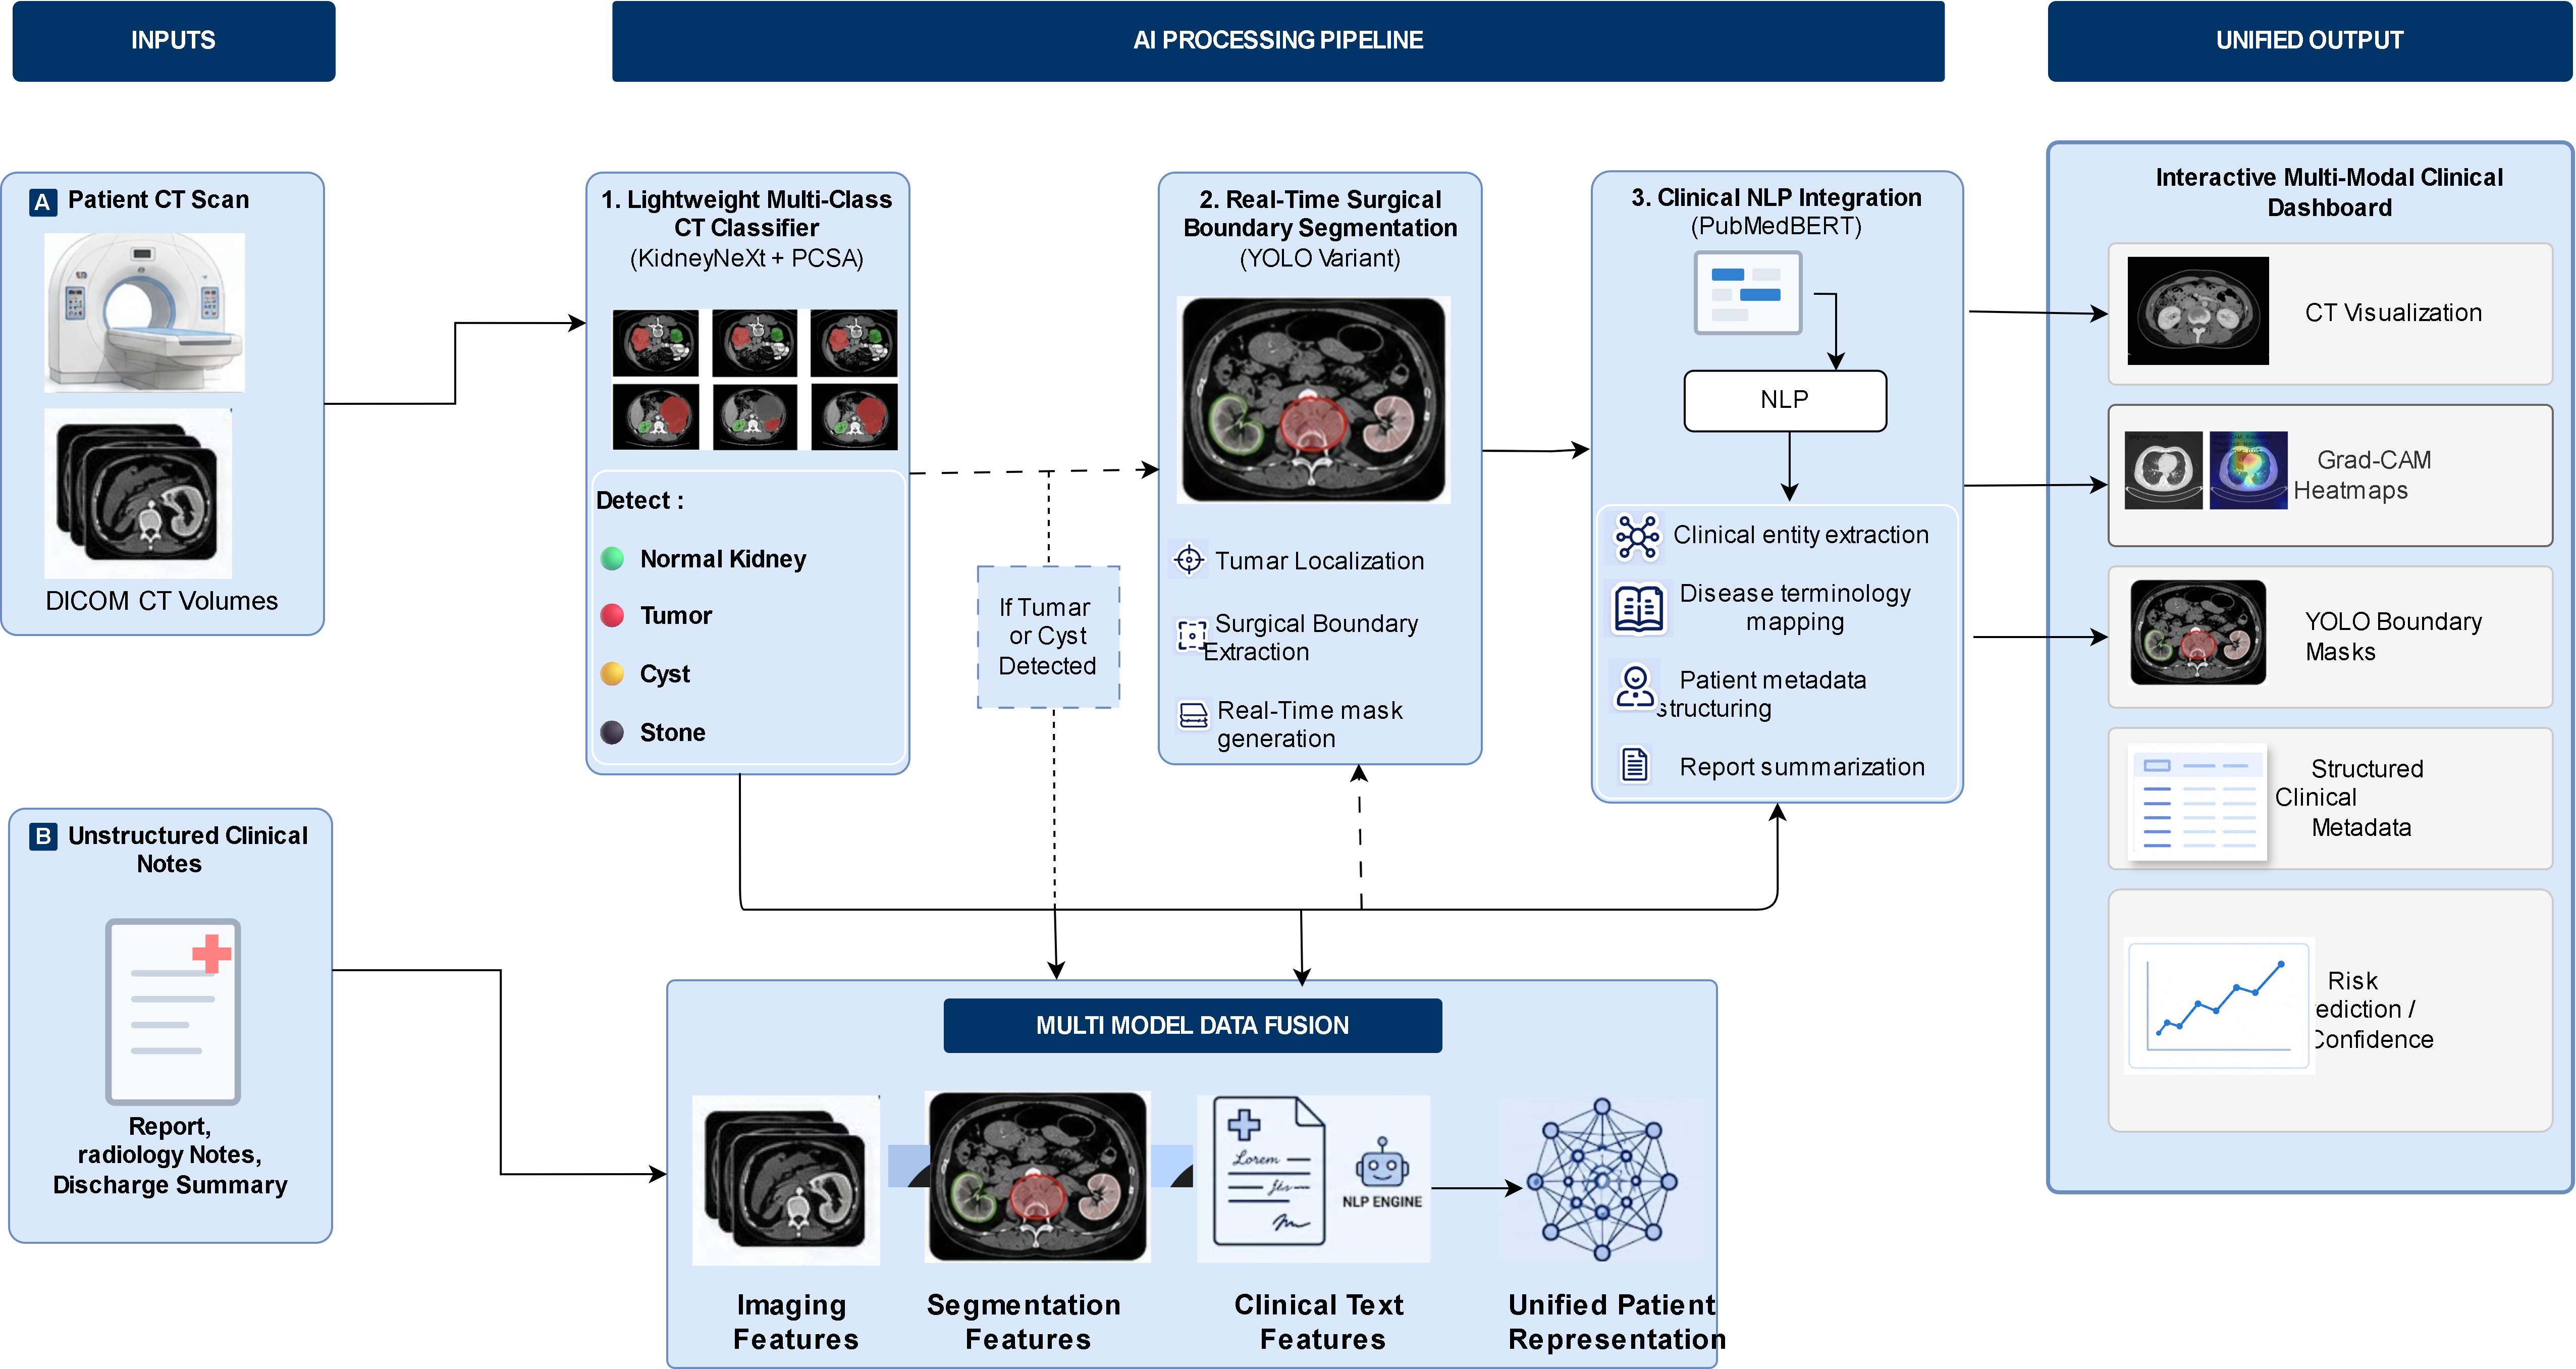
\includegraphics[width=\textwidth]{images/pipeline.png}
\caption{\textbf{Proposed Unified Clinical Pipeline.} The theoretical three-stage multimodal framework integrates lightweight CT classification for rapid triage (Stage~1), YOLO-based real-time boundary segmentation triggered by critical findings (Stage~2), and PubMedBERT-driven clinical NLP for automated report generation (Stage~3). All outputs converge in an interactive clinical dashboard.}
\label{fig:framework}
\end{figure*}

\subsection{Stage 1: Automated Renal Pathology Classification}
\label{subsec:stage1_classification}

The first stage functions as a high-throughput triage gate. Hospital Picture Archiving and Communication Systems (PACS) process substantial daily imaging volumes, and the practical viability of any AI-assisted workflow depends on architectures lightweight enough to operate within standard clinical computational budgets. Drawing on the KidneyNeXt backbone augmented with Pyramid Channel and Spatial Attention (PCSA) modules~\cite{alqahtani2025kidneynext, tawfik2026pcsa}, this stage would theoretically perform rapid multi-class categorisation based on the benchmark capabilities of these architectures across the four clinically relevant renal pathology categories---normal parenchyma, complex cysts, calcified stones, and solid malignancies---on standard 12,446-image CT datasets. 

Critically, this classification stage is not an end-point but a gating mechanism. Normal findings are logged and discharged from further processing; critical findings---tumour or obstructing calculus detections---conditionally route the imaging data to Stage~2. This conditional architecture ensures that computationally expensive segmentation resources are deployed selectively, preserving system throughput without sacrificing diagnostic coverage.

\subsection{Stage 2: Real-Time Surgical Boundary Segmentation}
\label{subsec:stage2_segmentation}

Preoperative planning for robot-assisted partial nephrectomy or PCNL demands spatial precision that extends well beyond what classification outputs provide. Surgeons require exact tumour margins, stone dimensions, and proximity to collecting system structures to minimise parenchymal sacrifice and reduce vascular complication risk. This stage addresses that need through real-time instance segmentation, proposing YOLOv11-based architectures adapted for medical imaging~\cite{akhtar2026yolov11}.

The case for a YOLO-family approach over traditional 3D U-Nets rests on practical clinical deployment constraints. While architectures such as ASD-Net~\cite{ji2024asdnet} or the spatial-channel attention enhanced U-Net~\cite{gohil2024kidney} deliver strong Dice performance on KiTS benchmarks, their 3D volumetric convolutions introduce inference latencies that are incompatible with real-time surgical guidance. A streamlined single-stage detector, operating on axial CT slices with CBAM-augmented attention, translates bounding box predictions into actionable surgical boundary masks at frame rates appropriate for intraoperative use, delivering the low-latency spatial feedback that the clinical environment demands.

\subsection{Stage 3: Clinical NLP Integration}
\label{subsec:stage3_nlp}

The third stage addresses a dimension of clinical AI that the imaging literature has largely treated as peripheral: the structured representation of unstructured clinical knowledge. Radiological reports, referring physician notes, and laboratory results contain contextual information---prior stone episodes, family history of renal cell carcinoma, eGFR trajectories---that no amount of CT pixel analysis can replicate. Integrating this textual context into the diagnostic workflow requires domain-adapted biomedical language models.

By deploying PubMedBERT~\cite{gu2021domain} fine-tuned for clinical Named Entity Recognition (NER), this stage would theoretically ingest the unstructured patient health record alongside the visual metadata produced in Stages~1 and~2. The NLP engine extracts structured clinical entities---pathology type, anatomical location, relevant comorbidities, and urgency indicators---and maps them against the imaging findings. A confirmed 3~cm lower-pole renal mass, when cross-referenced with a clinical note documenting haematuria and elevated creatinine, yields a materially different management recommendation than the same imaging finding in an asymptomatic screening context. This multimodal synthesis is precisely the integration that current literature identifies as absent from deployed renal AI systems~\cite{sreenivas2025enhancing}.

\subsection{The Integrated Clinical Dashboard}
\label{subsec:unified_dashboard}

The technical outputs of the three stages described above are clinically meaningful only if they are accessible and interpretable at the point of care. The proposed dashboard consolidates four information streams into a single interface: the original DICOM CT slice; the Grad-CAM interpretability overlay from Stage~1; the YOLO-generated surgical boundary masks from Stage~2; and the structured clinical metadata compiled by Stage~3. This co-presentation is deliberate---it enables the reviewing nephrologist or urologist to cross-validate the automated findings against the original imaging and the patient's clinical context without navigating multiple systems.

The design principle underlying this dashboard is epistemic transparency: every automated output is accompanied by its visual justification, and the clinician retains final authority at each decision point. This architecture directly addresses the accountability concerns raised in Section~\ref{sec:xai}, embedding XAI not as a post-development afterthought but as a structural component of the clinical interface. Integration with HL7 FHIR standards ensures that dashboard outputs feed directly into existing hospital information systems, avoiding the manual transcription overhead that represents one of the most persistent barriers to AI adoption in clinical settings~\cite{liang2025multicenter}.

% SECTION 7: REAL-WORLD DEPLOYMENT CHALLENGES

\section{Real-World Deployment Challenges}
\label{sec:challenges}

Demonstrating strong performance on curated benchmark datasets is a necessary but insufficient condition for clinical deployment. The gap between a model that achieves 99\% accuracy on the Kaggle CT Kidney dataset and one that functions reliably across the heterogeneous conditions of a busy district general hospital is substantial, and the literature has only recently begun to address it systematically. This section examines the three most consequential barriers: distributional generalisation, the mismatch between algorithmic and clinical metrics, and the engineering complexity of PACS integration.

\subsection{Data Generalisation and Modality Shifts}
\label{subsec:generalization_shifts}

The majority of high-performing renal AI models are trained and validated on a small number of well-curated repositories. The Kaggle CT Kidney dataset~\cite{ahmed2021ct, hossain2025detection} and the KiTS challenge cohorts~\cite{heller2023kits21} have been invaluable for establishing algorithmic baselines, but their controlled acquisition conditions do not reflect the scanner heterogeneity encountered in routine clinical imaging. Slice thickness, reconstruction kernel, contrast phase, and vendor-specific HU calibration all vary substantially across institutions, and these variations systematically degrade model performance in ways that benchmark evaluations do not capture~\cite{abdelrahman2022deep}. 

This reliance on homogeneous training data or single-modality captures is a prevalent limitation observed across a broad spectrum of current multi-task, super-resolution, and volumetric segmentation literature~\cite{abdalla2025axial, ma2022flare, macin2025kidneynext, xie2020seru, nguyen2025super, gao2026multitask, chen2023glunet, sherryl2022ied}.

The multi-phase nature of renal CT protocols compounds this problem. Models trained primarily on portal venous or nephrographic phase acquisitions frequently fail on non-contrast studies, where calculi are most visible but soft-tissue contrast is limited, and on arterial phase acquisitions, where vascular anatomy introduces confounding HU patterns~\cite{liang2025multicenter, ye2026automated}. Without prospective multi-centre validation incorporating the full range of acquisition protocols encountered in clinical practice, published performance figures should be interpreted with caution. The models reviewed in this survey that explicitly report external validation---notably the multi-centre 3D CNN of Liang et al.~\cite{liang2025multicenter} and the DBAR-Net of Sharon and Anbarasi~\cite{sharon2025attention}---represent the direction that the field must move, but they remain the exception rather than the rule.

\subsection{Algorithmic vs.\ Clinical Metrics}
\label{subsec:metrics_gap}

The standard performance vocabulary of deep learning---Dice Similarity Coefficient, Intersection over Union, macro F1-score---was designed to measure spatial or categorical alignment between model outputs and annotated ground truth. These metrics are well-suited to comparing architectures on a fixed dataset, but they are poor proxies for the outcomes that matter clinically.

Consider a model that achieves a Dice score of 0.92 on kidney tumour segmentation. That figure may reflect near-perfect delineation of a large, well-defined clear cell carcinoma while entirely missing a 4~mm satellite lesion at the tumour margin---a miss that has negligible impact on the aggregate score but significant implications for resection completeness~\cite{raj2022deep, gohil2024kidney}. Equally, a stone detection model reporting 96\% accuracy may perform adequately on stones larger than 5~mm while failing on sub-3~mm calculi that are clinically relevant for PCNL access planning~\cite{ye2026automated}. The disconnect is systematic: optimising for pixel-level metrics during training does not guarantee that the resulting model behaviour aligns with surgical priorities.

Addressing this requires a fundamental shift in how renal AI is evaluated. Clinical validation studies should incorporate task-specific metrics: stone-free rate prediction, surgical margin clearance rates, reduction in time-to-report, and inter-observer variability across radiologist cohorts~\cite{noorelahi2025pacs}. Progress in this direction is slow---partly because such endpoints require prospective clinical trial infrastructure---but it is a prerequisite for regulatory approval and sustainable clinical adoption.

\subsection{PACS Integration and Computational Overhead}
\label{subsec:pacs_integration}

Even a model that satisfies both generalisation and clinical validity requirements faces a third class of challenge: the practical engineering of integration into legacy hospital infrastructure. Most deployed clinical imaging systems were not designed with deep learning inference in mind, and retrofitting AI processing into existing PACS workflows introduces non-trivial latency, data governance, and interoperability constraints.

Large-scale 3D architectures---volumetric U-Net variants, multi-scale Vision Transformers---typically require enterprise-grade GPU hardware (e.g., NVIDIA A100 or Tesla-class accelerators) to maintain inference speeds compatible with clinical workflows~\cite{azad2023daeformer, li2022automatic}. The majority of district-level clinical environments lack this infrastructure, and even where it exists, the overhead of routing DICOM data to GPU-equipped inference servers introduces latency that may be unacceptable for time-sensitive applications such as emergency renal colic triage~\cite{ye2026automated}. Model compression techniques---quantisation, knowledge distillation, and pruning---offer partial mitigation, but their application to medical imaging models requires careful validation to ensure that compression does not disproportionately degrade performance on the rare but clinically critical edge cases~\cite{kadhim2024machine}.

Interoperability presents a parallel challenge. Clinical AI outputs must be delivered in formats that integrate natively with hospital information systems and downstream documentation workflows. The HL7 FHIR standard provides a structured mechanism for this integration, and its adoption by frameworks such as the multi-centre urinary disease detection system of Liang et al.~\cite{liang2025multicenter} demonstrates that PACS-compatible deployment is achievable. Scaling this approach across diverse institutional environments, each with different legacy system configurations, nonetheless remains a substantial engineering undertaking that the research community has yet to address systematically~\cite{ali2024comprehensive}.

% SECTION 8: CONCLUSION


\section{Conclusion}
\label{sec:conclusion}


\subsection{Summary of Findings}
\label{subsec:summary}

This survey has traced the progression of deep learning in renal imaging from early CNN-based multi-class classifiers through to the current generation of hybrid Vision Transformer and attention-augmented architectures. Several clear trajectories emerge from the literature. First, raw classification and segmentation accuracy---while still improving---is no longer the primary differentiator between architectures; the field is increasingly stratified by computational efficiency, architectural interpretability, and demonstrated robustness to domain shift. Second, the adoption of Explainable AI has moved from optional enhancement to practical necessity: models deployed in surgical planning contexts without transparent decision mechanisms face significant barriers to clinical acceptance, regardless of their benchmark performance. Third, and most significantly, the prevailing model-centric framing of renal AI---in which each architecture is evaluated in isolation on a static dataset---is increasingly misaligned with the integrated, multimodal nature of actual clinical workflows.

The reviewed literature also reveals persistent structural gaps. Multi-centre external validation remains rare. Clinical outcome metrics are seldom reported alongside algorithmic ones. NLP integration with imaging pipelines is largely theoretical in existing publications. These gaps are not incidental; they reflect the boundary between what is tractable as a machine learning problem and what is required for clinical translation.

\subsection{Clinical Outlook}
\label{subsec:outlook}

The trajectory of renal AI points unambiguously toward multimodal integration. The isolated successes documented across classification, segmentation, and language modelling are necessary precursors, but they become clinically transformative only when composed into coherent diagnostic pipelines. The unified framework proposed in Section~\ref{sec:framework} represents one such composition: a sequentially coupled system in which lightweight classification gates downstream segmentation, segmentation outputs inform report generation, and all findings are presented through an interpretable, PACS-integrated interface.

Realising this vision requires progress on multiple fronts simultaneously---generalisation, evaluation methodology, and systems engineering---none of which can be solved by algorithmic innovation alone. It demands prospective clinical collaborations, standardised benchmarking protocols, and regulatory frameworks adapted to the iterative nature of deployed AI. The role of the nephrologist and urologist in this process is not diminished by automation; it is recentred. Human clinical judgment remains the validating authority for AI outputs, and designing systems that honour that authority---through transparency, appropriate uncertainty communication, and genuine human override capacity---is the most consequential design challenge facing renal AI today.